\myChapter{Remoting Layer}\label{chap:remotinglayer}
Eine besondere Form des Presentation Layer ist der Remoting Layer, der die
Aufgabe übernimmt eine Anwendung über verscheidene \ac{RPC} Protokolle
anzubinden. In diesem Kapitel soll zuerst ein zentralisierter
Ausführungsmechanismus vorgestellt werden, der eine verallgemeinerte Form eines
\ac{RPC} Aufrufs annehmen kann. Anschließend werden konkrete \ac{RPC} Protokolle
und deren Implementierungen besprochen, die einen Aufruf in diese Form umwandeln
können.

\section{Service Engine}\label{sec:serviceengine}
Im Service Layer werden eine Reihe von Java Interfaces bereitgestellt, welche die
nach außen hin sichtbare Schnittstelle einer Anwendung definieren. Da die Service
Methoden so kompakt wie möglich gehalten werden sollten und nur die Methoden
bereitgestellt werden, die auch tatsächlich von den Benutzern verwendet werden,
eignen sich diese Interfaces auch als Schnittstelle für entfernte Methodenaufrufe
(vgl. \cite{fowler:2002} S. 135).

Zu diesem Zweck existieren in Java eine Reihe von Bibliotheken, die verschiedene
\ac{RPC} Protokolle implementieren. Jede Bibliothek verfolgt dabei ein eigenes
Konzept, wie ein Service in dem entsprechendem \ac{RPC} Protokoll zur Verfügung
gestellt wird. Möchte man eine Schnittstelle über verschiedene Protokolle zur
Verfügung stellen ist es notwendig, jede Bibliothek individuell zu
konfigurieren, obwohl die dafür notwendigen Informationen jeweils identisch sind. Gleichzeitig
fehlt ein zentraler Ausführungsmechanismus, da jede \ac{RPC} Bibliothek die
Ausführung der aufgerufenen Methoden selbst übernimmt.

Diesen Nachteilen soll die Zwischenschicht der Service Engine entgegenwirken,
indem sie die Verwaltung aller vorhandenen Services und die zentrale Ausführung
von Methoden übernimmt, ohne selbst ein \ac{RPC} Protokoll zu implementieren.
Implementierungen eines Protokolls (anschließend \emph{Protocol Handler} genannt)
sind dann die der Service Engine übergeordneten Schichten. Sie müssen lediglich
die Konvertierung eines konkreten \ac{RPC} in eine allgemeine Form übernehmen, die
dann an die Service Engine zur Ausführung übergeben werden kann.

Einzuordnen ist die Service Engine als Zwischenschicht direkt über dem Service
Layer, befindet sich aber bereits in der vormals eingeführten Remoting Schicht
(siehe Abbildung \ref{ill:serviceengine}).

\begin{figure}[bth]
    \center{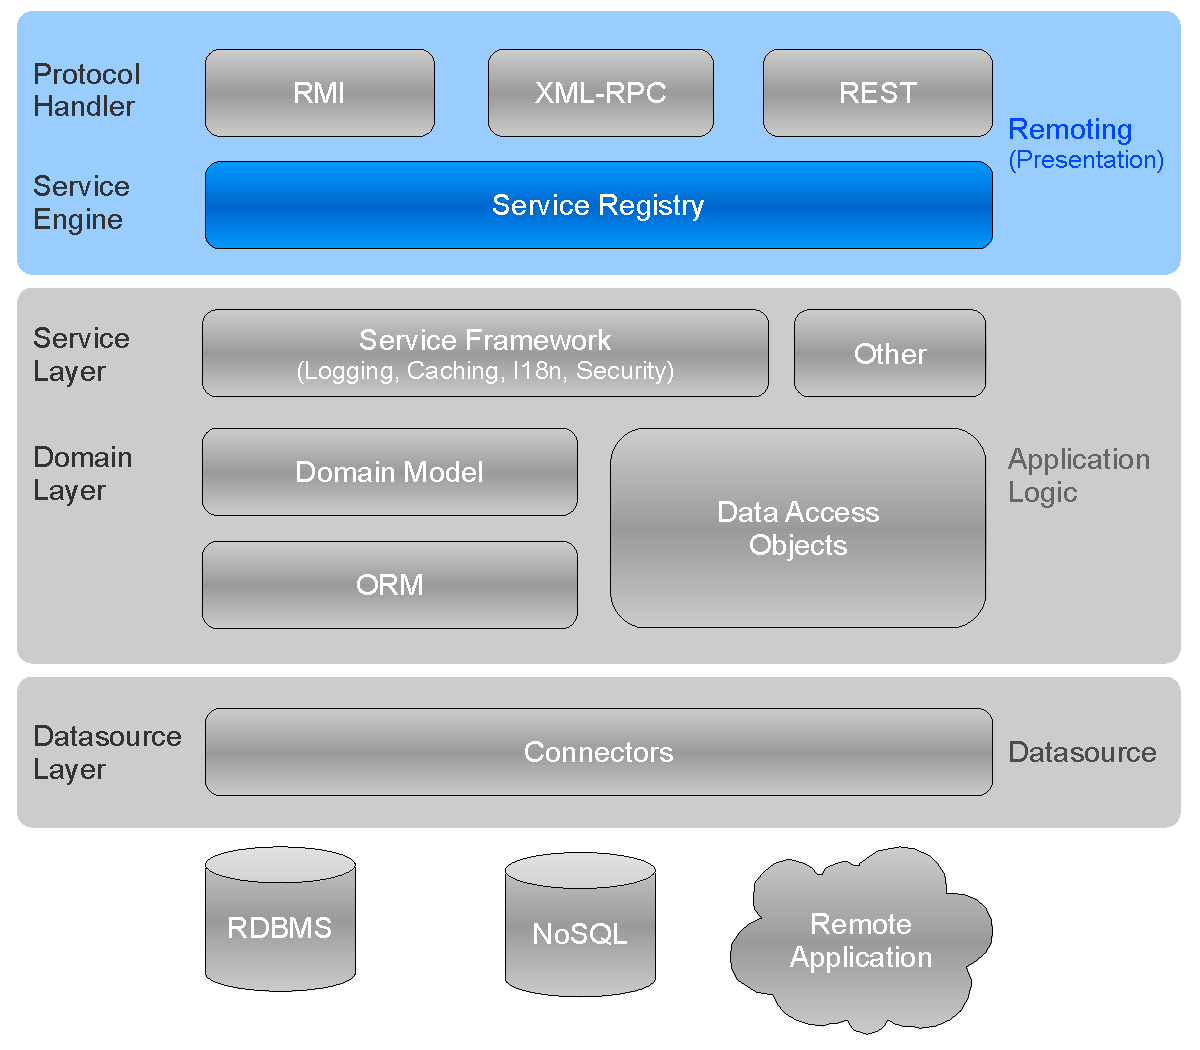
\includegraphics[width=\linewidth]{images/overviews/serviceengine}}
	\caption{Einordnung der Service Engine}
	\label{ill:serviceengine}
\end{figure}

\subsection{Remote Schnittstelle}
Das Konzept des Service Layer sieht vor, dass sich die Service Methoden direkt
nach den Anforderungen der Benutzer richten. Als direkt übergeordnete Schicht ist
auch die Service Engine ein Benutzer des Service Layer und kann deshalb ebenfalls
auf die Erstellung der Service Layer Schnittstelle Einfluss nehmen. Dabei
richten sich die Anforderungen der Service Engine wiederum nach den Protocol
Handlern und den \ac{RPC} Protokollen, die diese implementieren. Obwohl der
Service Layer keine direkten Abhängigkeiten von seinen übergeordneten Schichten
haben sollte, wirken sich die unterstützten \ac{RPC} Protokolle somit trotzdem
indirekt auf die Implementierung des Service Layer aus.

Nicht alle \ac{RPC} Protokolle stellen dabei den gleichen Funktionsumfang zur
Verfügung. Das erste wichtige Unterscheidungsmerkmal ist, ob ein \ac{RPC} mit
Objekten und Methodenaufrufen arbeitet oder einfache Prozeduraufrufe übertragen
werden. Im letzteren Fall muss der Service Layer entsprechend so gestaltet
werden, dass die einzelnen Service Methoden wie getrennte Prozeduren ausgeführt werden
können, die nicht zu einem Objekt gehören. Ein weiterer zu beachtender Punkt ist,
ob ein \ac{RPC} Protokoll zustandsgebunden oder zustandslos arbeitet.
Zustandsgebunden heißt auch, dass ein Client über verschiedene Anfragen das
gleiche Service Objekt zur Verfügung hat, während bei einem zustandslosen Protokoll jede
Anfrage unabhängig von allen anderen Anfragen und ohne einen globalen Zustand
bearbeitet wird\footnote{Das bedeutet normalerweise, dass für jede Anfrage ein
neues Service Objekt erzeugt wird}.

Bei dem Entwurf und der Implementierung der Service Interfaces, die über die
Service Engine angebunden werden sollen, muss also der "`kleinste gemeinsame
Nenner"' zwischen den anzubietenden \ac{RPC} Protokollen gefunden werden. In
Abschnitt \ref{sec:protocolhandler} werden diese Einschränkungen an den dort
vorgestellten \ac{RPC} Protokollen näher analysiert.

\subsection{Service Registry}
Der zentrale Bestandteil der Service Engine ist das Interface der \emph{Service
Regitry}. Die Service Registry übernimmt die Verwaltung der Service Interfaces,
die Instanziierung entsprechender Objekte, sowie die zentrale Ausführung von
Methoden auf diesen Objekten. Jedem Service Interface ist hierbei ein eindeutiger
Name zugewiesen. Wie die Services verwaltet und instanziiert werden, bleibt
dabei der Klasse überlassen, die das Service Registry Interface implementiert. 

Da andere Teile der Implementierung bereits auf dem Spring Framework basieren,
hat es sich angeboten eine Service Registry zu implementieren, die auf dem
\emph{Application Context} des Dependency Injection Containers basiert. Die
Instanziierung und Benennung von Service Objekten wird hier bereits bei der
Erstellung des Spring Context vorgenommen. Die Implementierung des Service
Registry Interface in Form der \emph{ApplicationContextRegistry} stellt nun alle
Objekte aus einem Application Context als Service Objekte bereit, sofern sie nach
einer festgelegten Namenskonvention benannt sind. In der Standardeinstellung
werden alle Objekte, deren Name auf "`Service"' endet, über die Service Registry
verfügbar gemacht. Da diese Endung in der Service Registry eine redundante
Information darstellen würde, wird sie entfernt um daraus den eindeutigen Namen
für den bereitgestellten Service zu generieren. Beispielsweise ist das Context
Objekt "`userService"' dann in der Service Registry unter dem Namen "`user"'
verfügbar. Die Zuordnung von Objekten aus dem Application Context zu einem
Service Interface muss manuell vorgenommen werden, da ein Objekt auch mehrere
Service Interfaces implementieren kann. Die für die Ausführung von Methoden
wichtigen Bestandteile der Service Registry sollen in den folgenden Abschnitten
näher erläutert werden.

\subsection{Interne RPC Darstellung}
Wie bereits erwähnt ist es nicht die Aufgabe der Service Engine, ein konkretes
\ac{RPC} Protokoll zu implementieren. Das bedeutet, dass die übergeordnete
Schicht der Service Engine einen Methodenaufruf in einer verallgemeinerten Form
zur Verfügung stellen muss. Da diese Schicht in erster Linie aus
verschiedenen \ac{RPC} Protocol Handlern besteht, die ebenfalls in Java
implementiert werden, bietet sich für die allgemeine Darstellungsform eines Methodenaufrufs
deshalb die Implementierung einer entsprechenden Java Klasse an. Diese Klasse
muss alle Informationen enthalten, die für die Ausführung
benötigt werden:

\begin{itemize}
  \item Den Namen des Service in der Service Registry
  \item Den Namen der aufzurufenden Methode
  \item Eine Liste der Methodenparameter
  \item Eine Liste der Parameter Typen
  \item Informationen über den serverseitigen Zustand des Client
\end{itemize}

In Java lässt sich der Typ eines Parameters zur Laufzeit anhand der Instanz des
Parameter Objekts bestimmten, muss deshalb also nicht getrennt gespeichert
werden. Der serverseitige Zustand eines Client wird im folgenden Abschnitt näher
behandelt.

Die \emph{RemoteProcedureCall} Klasse wurde als unveränderliches Klasse mit den
oben genannten Datenelementen implementiert. Ein RemoteProcedureCall Objekt dient
lediglich als Transferobjekt zwischen der Service Engine und der übergeordneten
Schicht. Die Validierung und eventuell
notwendige Konvertierung von Parametern erfolgt dann an zentraler Stelle in der
Service Registry und wird in Abschnitt \ref{subsec:dispatcher} genauer
betrachtet.

\subsection{Sessions}\label{subsec:sessions}
Bei einem \ac{RPC} wird zwischen zustandslosen und zustandsbehafteten Protokollen
unterschieden, was auch bei der Ausführung von Methoden in der Service Registry
beachtet werden muss. Für die zustandslose Kommunikation kann für jede Anfrage
auf der Service Registry ein neues Service Objekt erstellt werden, auf dem die
übergebene Methode ausgeführt wird. Im Gegensatz dazu muss sich ein Client bei
einer zustandsbehafteten Kommunikation zu Beginn bei dem Server authentifizieren.
Nach einer erfolgreichen Authentifizierung kann der Server alle nachfolgende
Anfragen des Client diesem wieder eindeutig zuordnen. Das bedeutet auch, dass der
Client üblicherweise erwartet, für alle folgenden Anfragen die jeweils gleiche
Instanz eines Service Objekts zur Verfügung zu haben. Der serverseitige Zustand
von Objekten, die über die zustandsgebundene Kommunikation einem einzigen Client
zugeordnet sind, soll nachfolgend \emph{Session} genannt werden.

Wie für die allgemeine Form eines \ac{RPC} die RemoteProcedureCall Klasse
entwickelt wurde, ist es auch für Sessions notwendig einen Ansatz zu
implementieren, der unabhängig von einem bestimmten \ac{RPC} Protokoll arbeitet.
Da die Umsetzung von Sessions in verschiedenen Protokollen unterschiedlich
gehandhabt wird, bleibt die Erstellung und Zuordnung einer Session dem jeweiligen
Protocol Handler überlassen, während die Verwaltung an zentraler Stelle in der
Service Registry erfolgt. Ein Session Objekt repräsentiert jeweils den
serverseitigen Zustand eines bestimmten Clients. Zur Zuordnung und Identifikation
besitzt jedes Session Objekt einen eindeutigen Bezeichner (\emph{Session ID}).
Aufgabe des Protocol Handler ist es nun, Anfragen eines Client mit der
entsprechenden Session ID zu verbinden, so dass die Service Registry den
korrekten serverseitigen Zustand für die Ausführung der Anfrage auswählen
kann.

Auch für die Implementierung von Sessions bietet das Spring Framework eine gute
Grundlage. Bei der Definition eines Objekts im Context kann angegeben werden,
über welchen Zeitraum (\emph{Scope}) eine Objektinstanz im Application Context
zur Verfügung stehen soll. Standardmäßig unterscheidet Spring hierbei zwischen
\emph{Singleton} und \emph{Prototype}. Ein Singleton Objekt wird bei der
Initialisierung des Application Context erstellt und ist über die gesamte
Laufzeit der Anwendung verfügbar. Wird eine Referenz auf das Objekt angefordert
handelt es sich also immer um die gleiche Instanz. Im Gegensatz dazu wird ein
Prototype Objekt für jede angeforderte Referenz neu erstellt. Durch die hohe
Flexibilität des Spring Frameworks ist es auch möglich eigene Scopes für
Objekte zu definieren. Diese Möglichkeit wurde bei der Implementierung
verwendet um einen Scope zu erstellen, der an jeweils ein Session Objekt der
Service Registry gebunden ist. Möchte man also ein Objekt aus dem Spring
Context für jeweils einen Benutzer verfügbar machen, muss es im Context mit
diesem Scope definiert werden.

\subsection{Methodenausführung}\label{subsec:dispatcher}
Nachdem nun ein allgemeines Transferobjekt für einen \ac{RPC} in Form der
RemoteProcedureCall Klasse implementiert wurde und auch zustandsgebundene
Protokolle mit Hilfe der Session Umgebung in der Service Engine einen
serverseitigen Zustand erhalten, ist die Service Registry nun in der Lage,
die Informationen aus einem RemoteProcedureCall Objekt in einen Methodenaufruf
auf einem Service Objekt umzusetzen.

Den Benutzern der Service Engine werden bei der Erstellung eines passenden
RemoteProcedureCall Objekts bewusst verschiedene Möglichkeiten gegeben, in
welcher Form die Methodenparameter übergeben werden können. Dadurch ist die
Verwendung der Service Engine weniger komplex und die Konvertierung und
Validierung von Parametern erfolgt an zentraler Stelle in der Service Registry.
Eine wichtige Rolle spielt dabei die in Kapitel \ref{subsec:assocequ} behandelte
Äquivalenz zwischen JavaBeans und Assoziativen Arrays. Viele \ac{RPC} Protokolle
benutzen für die Übertragung von Objekten ein Format, dass sich relativ leicht in
ein assoziatives Array (Map) deserialisieren lässt\footnote{Beispielsweise
\ac{JSON}}. Damit nicht jeder Protocol Handler die Umwandlung in ein passendes
JavaBean selbst übernehmen muss, wird die Konvertierung von einem assoziativen
Array in ein JavaBean von der Service Registry vorgenommen. Hierfür wurde
ein Algorithmus implementiert, der bei einem gegebenen assoziativen Array aus
einer Reihe von JavaBean Klassen die passendste Implementierung auswählt, diese
instanziiert und die Properties des JavaBean mit den entsprechenden Werten der
Map füllt. Die ausgewählte JavaBean Klasse ist diejenige, deren Eigenschaften
am genauesten mit den Schlüsseln der übergebenen Map übereinstimmen. Für die
Suche der auszuführenden Methode ergibts sich dann das folgende Vorgehen:

\begin{enumerate}
  \item Im ersten Schritt muss das Service Objekt bestimmt werden. Über den
  Namen des Service wird es entweder in der Service Registry neu erstellt oder,
  wenn eine Session Umgebung vorliegt und das Objekt mit dem gegebenen Namen
  dort vorhanden ist, aus einer Session geholt.
  \item Daraufhin wird überprüft, ob das Service Interface eine Methode
  besitzt, die bereits mit dem Namen und der exakten Signatur des übergebenen
  RemoteProcedureCall Objekts übereinstimmt. Aufgrund einer Beschränkung in der
  Java Reflection muss Polymorphie bei den Parametern manuell geprüft
  werden\footnote{\url{http://stackoverflow.com/questions/2169497/unexpected-class-getmethod-behaviour}}.
  Wurde eine Methode gefunden, wird sie auf dem Service Objekt ausgeführt. 
  \item Wurde keine passende Methode gefunden, werden alle Methoden mit dem
  Namen und der Anzahl von Parametern des RemoteProcedureCall Objekts gesucht.
  Nun wird für jeden Parameter überprüft, ob es sich um ein assoziatives Array
  handelt. Ist dies der Fall, wird unter allen Parameter Typen der Methoden an
  dieser Stelle das passendste JavaBean instanziiert. Mit diesen neu gewonnenen
  Parametern wird nun erneut Schritt zwei ausgeführt.
  \item Wurde keine Methode gefunden, wird eine NoSuchMethodError Exception
  geworfen. Als Erweiterung der Ausführungsvorgangs hat ein Service Objekt noch die
  Möglichkeit grundsätzlich alle Methodenaufrufe behandeln zu können, indem es
  das \emph{Interceptable} Interface implementiert. Wurde in den Schritten zwei
  und drei keine passende Methode gefunden, wird der Methodenaufruf an dieses
  Interface übergeben.
\end{enumerate}

\subsection{Übersicht}
Das \ac{UML} Diagramm in Abbildung \ref{ill:serviceengine_uml} zeigt die
wichtigsten an der Service Engine beteiligten Interfaces. Die Schnittstelle der
Service Engine zu übergeordneten Schichten besteht aus dem ServiceRegistry und
dem Session Interface sowie der RemoteProcedureCall Klasse. Das ProtocolHandler
Interface wird von Klassen implementiert, die eine Instanz einer Service Registry
benötigen.

\begin{figure}[bth]
    \center{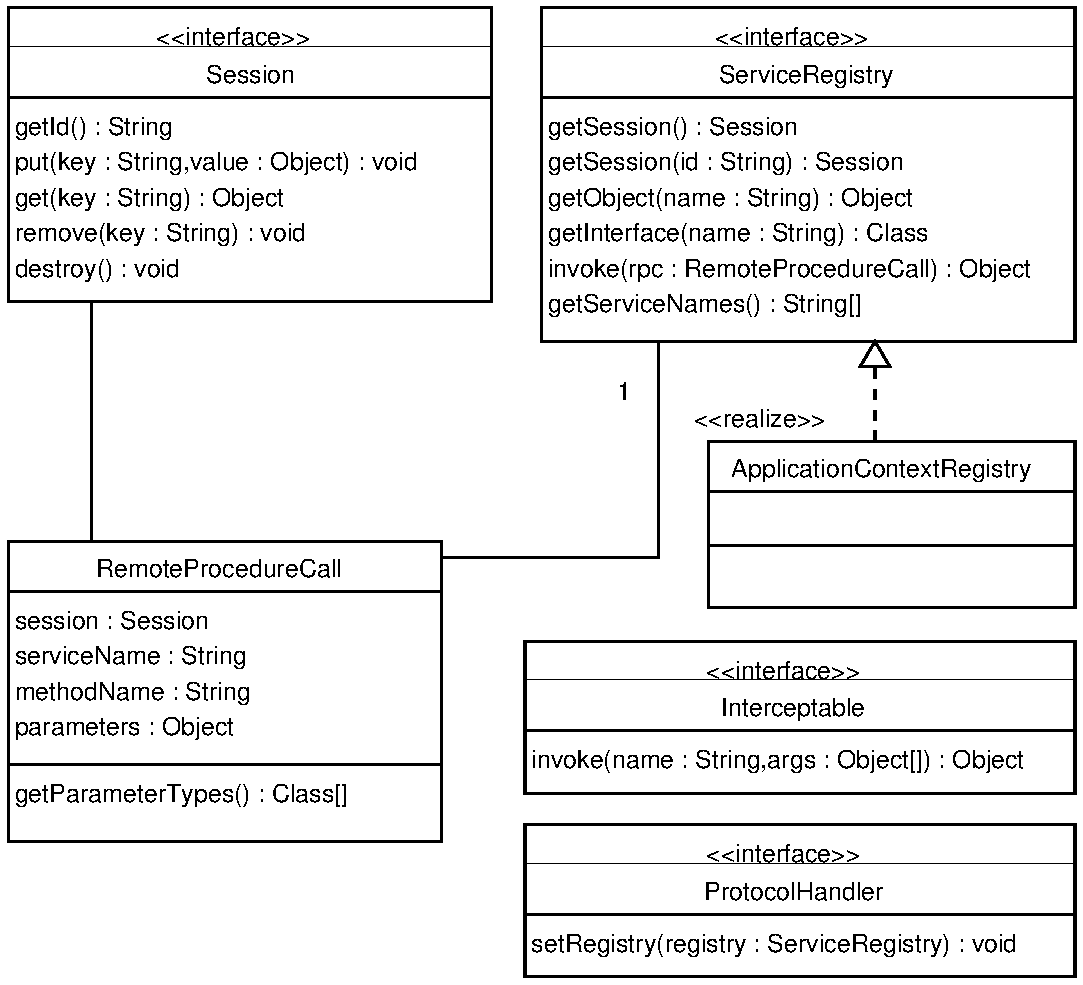
\includegraphics[width=\linewidth]{images/uml/serviceengine}}
	\caption{UML Diagramm der wichtigsten Komponenten der Service Engine}
	\label{ill:serviceengine_uml}
\end{figure}

\pagebreak
\section{Protocol Handler}\label{sec:protocolhandler}
Die Service Engine stellt über die Schnittstelle der Service Registry eine
Möglichkeit zur Verfügung, einen \ac{RPC} in der allgemeinen Form des
\emph{RemoteProcedureCall} Objekts ausführen zu können. Es ist nun die Aufgabe
der \emph{Protocol Handler}, die tatsächliche Implementierung der verschiedenen
\ac{RPC} Protokolle bereitzustellen und der Service Registry in Form dieses
Objekts zur Ausführung zu übergeben. Die Aufgaben eines Protocol Handler umfassen
somit:

\begin{itemize}
  \item Beschreibung der Java Interfaces in der \ac{IDL} des
  implementierten \ac{RPC} Protokolls, soweit notwendig. Für die meisten
  \ac{RPC} Protokolle beinhaltet das Java Service Interface bereits alle
  Informationen, die für die Schnittstellenbeschreibung notwendig sind.
  \item Bereitstellung eines Namensdienstes zur Auffindung der Services
  einer Service Registry, soweit nowendig.
  \item Annahme von Anfragen in einem spezifischen \ac{RPC} Protokoll.
  \item Initialisierung einer zu dem \ac{RPC} Protokoll gehörigen Session
  Umgebung.
  \item Deserialisierung von Methodenaufrufen und Umwandlung in ein
  RemoteProcedureCall Objekt.
  \item Übergabe des RemoteProcedureCall Objekts an die Service Registry zur
  Ausführung des Methodenaufrufs.
  \item Serialisierung des Ergebnisses in das Austauschformat des \ac{RPC}
  Protokolls und Übertragung dieser Daten.
  \item Serialisierung von Fehlern, die während der Methodenausführung
  aufgetreten sind.
\end{itemize}

In der Gesamtarchitektur sind die Protocol Handler im Remoting Layer über der
Service Engine einzuordnen (siehe Abbildung \ref{ill:protocolhandler}). Es ist
die Schicht des Gesamtsystems, mit der andere entfernte System direkt
kommunizieren.

\begin{figure}[bth]
    \center{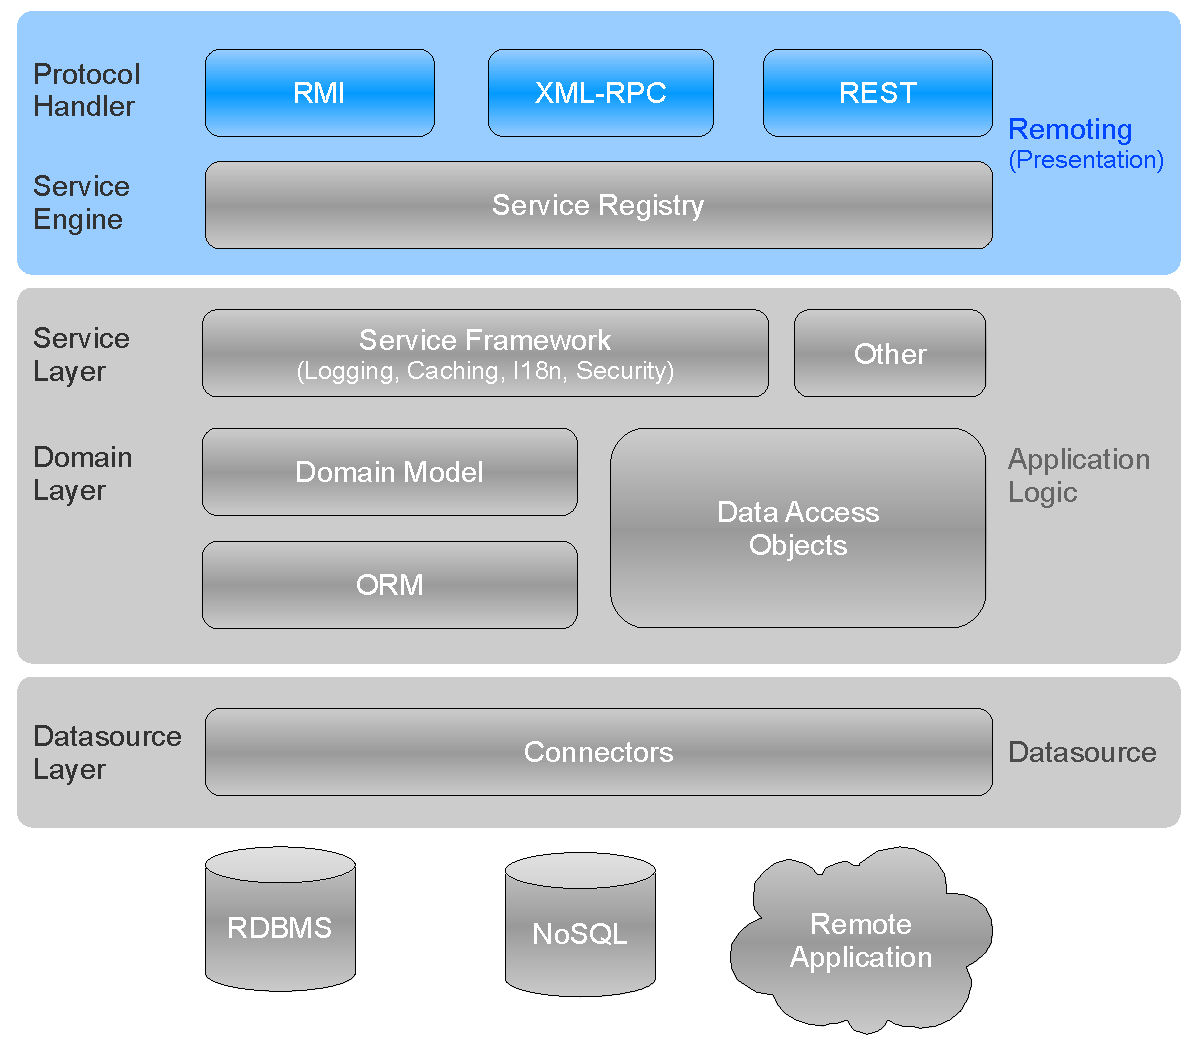
\includegraphics[width=\linewidth]{images/overviews/protocolhandler}}
	\caption{Einordnung der Protocol Handler}
	\label{ill:protocolhandler}
\end{figure}

Es ist weiterhin möglich, die Implementierungen vorhandener \ac{RPC} Protokolle
zu verwenden, so lange die Möglichkeit besteht, Methodenaufrufe in die
abstrahierte Form des RemoteProcedureCall Objekts zu konvertieren und an die Service Registry
zu übergeben. In diesem Kapitel sollen drei unterschiedliche \ac{RPC} Protokolle
und deren Implementierungen eines Protocol Handler vorgestellt werden. Die
ausgewählten Protokolle verfolgen jeweils unterschiedliche Ansätze bezüglich
serverseitigem Zustand und der Art von Methoden- bzw. Prozeduraufrufen. Deshalb
sind sie gut geeignet, die Vorteile, die durch die Verwendung der Service Engine
entstehen, aufzuzeigen.

\subsection{Remote Method Invocation}\label{subsec:rmi}
Java \ac{RMI} (siehe \cite{sun:rmi}) ist die Implementierung eines binären
\ac{RPC} Protokolls für den Austausch von Objekten zwischen verschiedenen, auch
entfernten, Instanzen einer \ac{JVM}. Es setzt dabei stark auf die von der
\ac{JVM} unterstützten Serialisierung von Objekten. \ac{RMI} ist
zustandsgebunden, wodurch auch auf entfernten Objekten Methodenaufrufe
ausgeführt werden können. An der für \ac{RMI} notwendigen Infrastruktur sind
folgende Komponenten beteiligt (siehe \cite{wiki:rmi}):

\begin{description}
\item[Remote Interface] Das Remote Interface ist ein Java Interface, das dem
Client bekannt ist und die auf dem Server implementierten Methoden beschreibt.
Dadurch wird das Problem, die vom Server bereitgestellten Methoden zu
beschreiben, auf eine für Java natürliche Art und Weise gelöst.
\item[Remote Object] Das Remote Object ist eine Instanz der Klasse, die das
Remote Interface auf der Serverseite implementiert.
\item[RMI Registry] Die \ac{RMI} Registry ist ein Namensdienst, der für das
Auffinden der vom Server bereitgestellten Remote Objekte zuständig ist. Jeweils
einem implementierten Remote Interface wird dabei ein eindeutiger Name
zugewiesen.
\item[Remote Reference] Erkundigt sich der Client bei der \ac{RMI} Registry nach
dem Remote Object für einen bestimmten Namen, bekommt er eine Referenz auf das
serverseitige Remote Object zurück.
\end{description}

Ist die Verbindung von einem Client zu einem Remote Object auf dem Server
hergestellt, erlaubt \ac{RMI} eine transparente Kommunikation. Auch
Klassendefinitionen, die auf der jeweils anderen Teilnehmerseite nicht
vorhanden sind, werden dynamisch nachgeladen. Tritt einer der bei einem
\ac{RPC} zusätzlichen Fehlerfälle auf, wird eine \emph{RemoteException}
geworfen. Abbildung \ref{ill:rmi} zeigt den Ablauf der \ac{RMI}
Kommunikation und den beteiligten Komponenten.

\begin{figure}[bth]
	\center{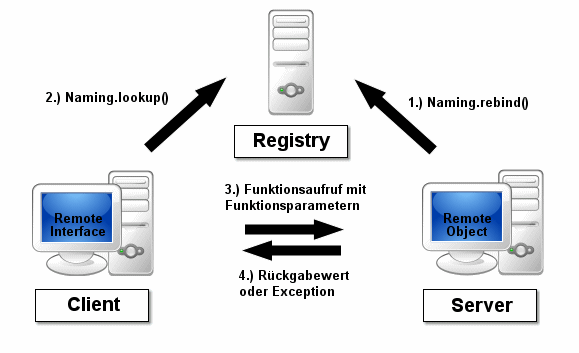
\includegraphics[width=\linewidth]{images/rmischema}}
	\captionof{figure}[RMI Kommunikation]{Kommunkationsablauf bei
	RMI\footnotemark}
	\label{ill:rmi}
\end{figure}
\footnotetext{Quelle: \cite{wiki:rmi}, Public Domain}

\subsubsection{Spring und RMI}
Das Spring Framework vereinfacht die Nutzung von \ac{RMI} erheblich (vgl.
\cite{spring:reference} Abschnitt 19.2). So können in einem Kontext definierte
Objekte ebenfalls über eine Context Konfiguration als \ac{RMI} Services
exportiert werden, wenn sie das zu exportierende Remote Interface implementieren.

Da das Spring Framework durch Dependency Injection bereits die Verwendung von
Interfaces unterstützt, muss im Spring Context der Clientseite dann lediglich
ein \emph{Proxy} definiert werden, der das Remote Interface für den Client
implementiert und mit dem im Context angegeben \ac{RMI} Server
kommuniziert. Für Klassen des Client, die das Remote Interface verwenden, wird
dann dieser Proxy injiziert.

Listings \ref{lst:rmiserver} und \ref{lst:rmiclient} zeigen eine Spring Context
Konfiguration für die Verwendung des in Abschnitt \ref{service:i18n}
vorgestellten I18NService über \ac{RMI}.

\lstset{language=xml}
\lstinputlisting[caption=Spring und RMI - Server Context,
label=lst:rmiserver]{sources/springrmiserver.xml}

\lstinputlisting[caption=Spring und RMI - Client Context,
label=lst:rmiclient]{sources/springrmiclient.xml}

\subsubsection{Implementierung}
Da Spring bereits eine sehr gute Unterstützung für \ac{RMI} besitzt ist es
sinnvoll die dafür verwendeten Klassen für die Implementierung eines \ac{RMI}
Protocol Handler zu erweitern. Die \emph{RmiProtocolHandler} Klasse erstellt so für jeden
in der Service Registry vorhandenen Service eine Instanz des Spring
\emph{RmiServiceExporter} mit den passenden Parametern für Service Name, Service
Instanz und Service Interface. Dadurch sind bereits alle Service Interfaces über
\ac{RMI} auffindbar.

Schwieriger gestaltet sich nun die Bereitstellung des passenden Remote Object.
Der Client ruft über das ihm bekannte Remote Interface eine Methode auf einem
serverseitigen Remote Object auf. Auf dem Remote Object selbst verhält sich
dieser Aufruf genauso wie ein lokaler Methodenaufruf. Die Aufgabe des Protocol
Handler ist es aber, diesen Aufruf in ein entsprechendes
\emph{RemoteProcedureCall} Objekt umzuwandeln. Um diese Umwandlung zu
realisieren, wird ein Service Interface von einem \ac{AOP} Proxy\footnote{Siehe Abschnitt
\ref{define:aop}} implementiert, der dann als Remote Object dient. Durch einen
\emph{Around Advice} für alle Methodenaufrufe auf diesem Proxy ist es nun
möglich, die Informationen des Methodenaufrufs zu extrahieren und in ein
\emph{RemoteProcedureCall} Objekt umzuwandeln, das dann an die Service Registry
übergeben werden kann. Auch die Identifikation der Session ist bei diesem
Vorgehen problemlos möglich, da ein Remote Object, also hier das Proxy Objekt,
immer direkt einem Client zugeordnet ist.

\subsection{XML-RPC}\label{subsec:xmlrpc}
XML-RPC ist ein zustandsloses \ac{RPC} Protokoll, das \ac{XML} als
Austauschformat und \ac{HTTP} als Übertragungsprotokoll verwendet (siehe
\cite{winer:1999}). Übertragen werden Prozeduraufrufe, wobei die Struktur bewusst
sehr einfach gehalten wird, weshalb das Protokoll sowohl auf Server- als auch auf
Clientseite leicht zu implementieren ist.

\subsubsection{Spezifikation}
Als Parameter- und Rückgabewerte werden sieben primitive und zwei
zusammengesetzte Typen unterstützt. Ein Typ wird jeweils von einem \emph{<value>}
XML Tag umschlossen. Die primitiven XML-RPC Typen sind in Tabelle
\ref{tab:xmlrpcprimitives} aufgelistet. Der zusammengesetzte Typ \emph{Struct}
ist das XML-RPC Äquivalent eines assoziativen Arrays, während der Typ
\emph{Array} eine geordnete Menge von beliebigen anderen XML-RPC Typen enthält. Im Fehlerfall
wird ein \emph{Fault} Objekt übertragen, das ein Struct Element mit den
Schlüsseln \emph{faultCode} und \emph{faultString} enthält.


\begin{table}[h] \begin{tabularx}{\textwidth}{lll} \toprule
   \tableheadline{Typ} & \tableheadline{XML Tag} &
    	\tableheadline{Beispiel} \\
   		\midrule Integer & <i4> oder <int> & <int>33</int>\footnotemark \\
    	Double & <double> & 3.1415 \\
    	Date/Time & <dateTime.iso8601> & 20100223T19:34:56 \\
    	Boolean & <boolean> & 1, 0, true, false \\ 
    	String & <string> & Text \\
    	Base64 Binärdaten & <base64> & VGV4dA== \\
		\bottomrule
	\end{tabularx}
\caption[XML-RPC primitive Typen]{Primitive Typen des XML-RPC Protokolls}
\label{tab:xmlrpcprimitives}
\end{table}
\footnotetext{In den weiteren Beispielen wurden die umschließenden XML Tags aus
Platzgründen weg gelassen}

Da XML-RPC \ac{HTTP} als Übertragungsprotokoll verwendet, erfolgt die
Lokalisierung über einen eindeutigen \ac{HTTP} \ac{URI}, wohin alle
Prozeduraufrufe gerichtet werden. Die XML-RPC Spezifikation sieht nicht vor, die zur Verfügung gestellten
Prozeduren automatisch zu beschreiben. Die Beschreibung erfolgt meist in Form
einer \ac{API} Dokumentation. Eine inoffizielle aber häufig verwendete
Erweiterung zur Schnittstellen Beschreibung ist die \emph{XML-RPC Introspection}
(siehe \cite{henderson:2007}).

Ein vollständiges Beispiel einer XML-RPC Kommunikation mit dem Aufbau von Struct,
Array und Fault Elementen sowie den dazugehörigen \ac{HTTP} Headern ist in
Anhang \ref{chap:appendix} zu finden.

\subsubsection{Implementierung}
Für Java existieren eine Reihe von Bibliotheken, die XML-RPC Anfragen verarbeiten
können. Deshalb bot es sich, an eine passende Implementierung für die Umsetzung
des XML-RPC Protocol Handler zu verwenden. Voraussetzung ist, dass die
Bibliothek die Möglichkeit bietet, eine eigene Implementierung für die
Bearbeitung eines deserialisierten XML-RPC zur Verfügung zu stellen. Nach der Evaluierung
verschiedener Bibliotheken fiel die Entscheidung dabei auf die \emph{Redstone
XML-RPC Library}\footnote{\url{http://xmlrpc.sourceforge.net/}}, da sie
performant arbeitet, klar strukturiert ist und eigene Erweiterungen zulässt. Für
die Realisierung musste dann lediglich ein Interface implementiert werden,
das bei einem XML-RPC Aufruf mit den entsprechenden Methodennamen und
Parametern aufgerufen wird. Dort wird dann das entsprechende
RemoteProcedureCall Objekt erstellt und an die Service Registry weitergegeben.

\subsection{Representational State Transfer}\label{subsec:rest}
Der Begriff \ac{REST} wurde von Roy T. Fielding im Jahr 2000 in
\cite{fielding:2000} (S. 76 - 106) geprägt und beschreibt einen Software
Architekturstil für verteilte Hypermedia Systeme. Hypermedia (vgl.
\cite{fielding:2000} S. 68) bedeutet die Verwendung von
\emph{Multimedia-Formaten} und \emph{Hypertext}\footnote{Beispielsweise in Form
von HTML oder XML} zur Übertragung von Informationen, wobei in einem
Hypertext-Dokument wiederum durch \emph{Hyperlinks} auf andere Hypermedia Inhalte
verwiesen werden kann. Verteilte Hypermedia Systeme erlauben es, diese Inhalte
auch von einem entfernten System zu beziehen.

Bei \ac{REST} handelt es sich um einen Architekturstil, also eine Richtlinie,
wie Anwendungen, die die für \ac{REST} festgelegten Kriterien erfüllen, strukturiert
werden können. Somit ist \ac{REST} selbst implementierungs- und
technologieunabhängig. Das bekannteste Beispiel einer Umsetzung des \ac{REST}
Architekturstils ist das \ac{HTTP} Protokoll, das im nachfolgenden Abschnitt
genauer behandelt wird. Anwendungen, die der \ac{REST} Architektur folgen,
werden auch als \emph{RESTful} bezeichnet. Damit eine Implementierung dem
\ac{REST} Architekturstil, folgt stellt Fielding verschiedene Bedingungen auf
(siehe \cite{fielding:2000} S. 76 - 85):

\begin{description}
  \item[Client-Server] Durch die Verwendung einer Client-Server Architektur ist
  eine einfache Trennung der Aufgabenbereiche (\emph{Separation Of Concerns}) für
  beide Teilnehmer möglich. Dabei ist der Client für die Darstellung zuständig,
  während der Server die Datenhaltung und die Anwendungslogik übernimmt.
  Verschiedene Clients können dabei die vom Server bereitgestellten Daten in
  unterschiedlichen Benutzeroberflächen bereitstellen und verarbeiten, während
  die serverseitige Anwendungslogik gleichzeitig vereinfacht werden kann. Ein
  weiterer Vorteil ist, dass beide Seiten unabhängig voneinander weiterentwickelt
  werden können, so lange sie das entsprechende Protokoll und Austauschformat
  einhalten.
  \item[Zustandslosigkeit] Die Kommunikation zwischen Client und Server erfolgt
  zustandslos. Das heißt, dass ein Client mit jeder Anfrage alle für die
  Bearbeitung der Anfrage notwendigen Informationen übertragen muss. Dadurch
  verringert sich die Komplexität der Serverseite weiter, da jede Anfrage
  unabhängig von einem globalen Zustand bearbeitet werden kann. Gleichzeitig
  wird die Skalierbarkeit erhöht, da jede Anfrage von einer beliebigen
  Serverinstanz bearbeitet werden kann.
  \item[Cache] Im Hinblick auf die Netzwerkauslastung kann sich eine zustandslose
  Kommunikation negativ auswirken, da viele Informationen mehrfach übertragen
  werden müssen. Deshalb sieht \ac{REST} die Verwendung von Caches vor. Ist die
  Antwort auf eine Anfrage des Client als cachebar gekennzeichnet, kann er diese
  in einem \emph{clientseitigem Cache} über einen bestimmten Zeitraum als Antwort
  für erneute, identische Anfragen verwenden. Auch die Verwendung von
  transparenten Caches (\emph{Proxies}) ist möglich.
  \item[Wohldefinierte Operationen] \ac{REST} sieht eine Reihe wohldefinierter
  Operationen vor, die auf Hypermedia Inhalten ausgeführt werden können. Die
  Identifikation und Beschreibung dieser Operationen wird im folgenden
  Abschnitt näher besprochen.
  \item[Schichtenarchitektur] Die schon in Kapitel \ref{chap:introduction}
  vorgestellten Vorteile einer Schichtenarchitektur finden auch in \ac{REST}
  Anwendung. In Verbindung mit der hier verwendeten einheitlichen Schnittstelle
  kann die nach außen hin sichtbare Komplexität eines Gesamtsystems erheblich
  reduziert werden.
  \item[Code-On-Demand] Code-On-Demand ist eine optionale Eigenschaft,
  die es erlaubt, einen Client um Funktionalitäten zu erweitern, die
  vom Server in Form eines Skripts oder Applets zur Verfügung gestellt werden. 
\end{description}

\subsubsection{Ressourcen}
Ein zentraler Bestandteil der \ac{REST} Architektur sind \emph{Ressourcen}.
Ressourcen können jede Art von Hypermedia Informationen sein, die eindeutig
addressierbar sind. Beispiele (vgl. \cite{fielding:2000} S. 88) sind ein
Dokument, eine Bilddatei, Listen von anderen Ressourcen, dynamische Services
(z.B. Wetterinformationen) oder Domain Objekte mit einem eindeutigen Bezeichner.
Bei verteilten Hypermedia Systemen geschieht die Addressierung in Form
eines \ac{URI}. In \cite{rfc3986}, der Definition des \ac{URI}, wird ein
einheitliches Addressierungsschema für Ressourcen festgelegt. Beispiele sind
(vgl. \cite{rfc3986} Abschnitt 1.1.2):
\begin{itemize}
  \item http://tools.ietf.org/html/rfc3986
  \item jdbc:mysql://host:port/database
  \item tel:+4989123456
  \item rmi://host:1099/serviceName
\end{itemize}
Vor allem in Verbindung mit dem \ac{HTTP} Protokoll wird oft der Begriff des
\ac{URL} verwendet. Die \ac{URL} Definition ist eine Untermenge der aktuelleren
\ac{URI} Spezifikation, weshalb im weiteren Verlauf der technisch korrekte
Begriff der \ac{URI} verwendet werden soll.

Nachdem nun Ressourcen eindeutig identifiziert werden können, müssen die darauf
auszuführenden Operationen definiert werden. In den meisten Fällen entsprechen
diese Operationen direkt einer \ac{CRUD} Schnittstelle.

\subsubsection{HTTP}\label{subsub:http}
\ac{REST} wurde aus den Design- und Implementierungsentscheidungen hergeleitet,
die bei der Entwicklung des \ac{HTTP} Protokolls maßgeblich waren. Bei \ac{HTTP}
handelt es sich somit um die am weitesten verbreitete und faktisch einzige (vgl.
\cite{tilkov:2009}) Implementierung des \ac{REST} Architekturstils. Im
Unterschied zu klassischen Webservices, die zwar \ac{HTTP} als
Übertragungsprotokoll verwenden, aber eine weitere Zwischenschicht für die
Nachrichtenübermittlung verwenden, verfolgt die \ac{REST} Umsetzung für \ac{HTTP}
den Ansatz, dass das \ac{HTTP} Protokoll selbst bereits alle dafür notwendigen
Eigenschaften besitzt.

\paragraph{HTTP Methoden}
Als Operationen, die auf allen Ressourcen ausgeführt werden können (siehe
\cite{rfc2616} Abschnitt 9), legt \ac{HTTP} \emph{GET},
\emph{POST}, \emph{PUT} und \emph{DELETE} sowie \emph{OPTIONS} und \emph{HEAD}
fest:

\begin{itemize}
  \item GET ist eine "`sichere"', nur lesende Methode,
  die die in der \ac{URI} festgelegte Ressource in einem vom Client gewählten Austauschformat
  zurückliefert. "`Sicher"' bedeutet hier, dass eine GET Operation nur lesend
  auf die Daten zugreift und in keinem Fall eine Veränderung auf der Serverseite
  bewirkt.
  \item PUT überträgt die Repräsentation einer Ressource, die an der von
  der \ac{URI} angegebenen Stelle angelegt werden soll. Die PUT
  Operation ist "`idempotent"'. Das bedeutet, dass sich mehrere identische PUT
  Operationen genauso auswirken wie eine einzige.
  \item DELETE löscht die von einer \ac{URI} angegebene Ressource.
  \item POST aktualisiert eine vorhandene Ressource. Außerdem können durch POST
  Operationen auch andere Methoden abgebildet werden. Über die tatsächliche
  Semantik einer POST Operationen entscheidet dabei die Serverseite.
  \item OPTIONS gibt Informationen über die vom Server unterstützten Methoden.
  Auch hierbei handelt es sich um eine sichere Operation.
  \item HEAD ist identisch zu einer GET Operation, außer dass lediglich der 
  \ac{HTTP} Header der Antwort gesendet wird.
\end{itemize}

\paragraph{Statuscodes}
Im Antwortheader jeder Anfrage gibt der Server verschiedene Statuscodes zurück,
die den Client darüber informieren, ob die Anfrage erfolgreich bearbeitet wurde
bzw. welche Fehler aufgetreten sind. Die dabei verwendeten Statuscodes sind in
verschiedene Bereiche (siehe \cite{rfc2616} Abschnitt 10) unterteilt, die in der
folgenden Tabelle \ref{tab:httpcodes} kurz beschrieben werden.

\label{tab:httpstatus}
\begin{table}[h]
	\begin{tabularx}{\textwidth}{lll} \toprule
    	\tableheadline{Bereich} & 
    	\tableheadline{Bedeutung} \\
    	\midrule
    	1xx & Informationen \\
    	2xx & Anfrage erfolgreich ausgeführt und bearbeitet \\
    	3xx & Weiterleitung, weitere Aktionen von Clientseite erwartet \\
    	4xx & Client Fehler, fehlerhafte Anfrage \\
    	5xx & Server Fehler, Anfrage kann nicht bearbeitet werden \\
		\bottomrule
	\end{tabularx}
	\caption{HTTP Statuscode Bereiche}
	\label{tab:httpcodes}
\end{table}

\paragraph{Content Negotiation}
Eine weitere für \ac{REST} wichtige Eigenschaft ist die Unterstützung von
verschiedenen Austauschformaten (\emph{Representations}) für eine Ressource. Zu
diesem Zweck unterstützt \ac{HTTP} die sogenannte \emph{Content Negotiation}.
Dadurch kann ein Client bei einer Anfrage im \emph{Accept} Teil des Headers
eine Liste der gewünschten Austauschformate angeben. Der Server antwortet dann
mit einer Repräsentation der Ressource in dem ersten Austauschformat aus der
Client Liste, dass er zur Verfügung stellen kann oder mit einem \emph{406 Not
Acceptable} Fehlercode, wenn die Darstellung der Ressource in keinem erwarteten
Format möglich ist.
 
\paragraph{Beispiel}
Das folgende Beispiel soll eine \ac{HTTP} Kommunikation veranschaulichen, die die
verschiedenen Methoden in Verbindung mit Content Negotation verwendet und dem
\ac{REST} Architekturstil folgt.

Ein Client sendet einen PUT Request für die Ressource \\
http://example.com/users mit der \ac{XML} Repräsentation einer Ressource an den
Server:
\lstset{language = Python}
\begin{lstlisting}[caption=HTTP PUT Request, label=lst:httpput]
PUT /users HTTP/1.1
Host: example.com
Content-Type: text/xml
Content-Length: 77
Accept: application/xml,application/json
Accept-Charset: ISO-8859-1,utf-8

<user>
	<username>UserX</username>
	<password>supersecret</password>
</user>
\end{lstlisting}
Daraufhin antwortet der Server mit einer passenden Statusmeldung, die im Feld
\emph{Content Location} die \ac{URI} der neu angelegten Ressource angibt:
\begin{lstlisting}[caption=HTTP PUT Antwort, label=lst:httpputeresp]
HTTP/1.1 201 Created
Date: Fri, 26 Feb 2010 11:39:07 GMT
Server: Service Engine HTTP Connector
Content-Location: http://example.com/users/2
\end{lstlisting}
\pagebreak
Nun kann ein anderer Client diese Resource in einem beliebigen vom Server
unterstützten Austauschformat anfordern:
\begin{lstlisting}[caption=HTTP GET Request, label=lst:httpget]
GET /users/2 HTTP/1.1
Host: example.com
Accept: application/json
Accept-Charset: utf-8,ISO-8859-1
\end{lstlisting}
Und bekommt die entsprechende Antwort:
\begin{lstlisting}[caption=HTTP GET Antwort, label=lst:httpgetresp]
HTTP/1.1 200 OK
Date: Fri, 26 Feb 2010 13:14:07 GMT
Server: Service Engine HTTP Connector
Content-Type: application/json; charset=utf-8
Content-Length: 55

{
	"username" : "UserX",
	"password" : "supersecret"
}
\end{lstlisting}

\subsubsection{Implementierung}
\ac{REST} ist kein \ac{RPC} Protokoll (vgl. \cite{fielding:2000} S. 141), da das
zentrale Element nicht Methodenaufrufe sondern Ressourcen sind, die über eine
gemeinsame, eindeutige Schnittstelle angesprochen werden können. Viele
Frameworks, die eine \ac{REST} Unterstützung über \ac{HTTP} anbieten, benötigen
deshalb zusätzliche Konfigurationseinstellungen, um die Zuordnung von Service
Methoden zu Ressourcen und \ac{HTTP} Methoden vornehmen zu können. Eine andere
häufig verwendete Möglichkeit ist ein Interface, das mit \ac{HTTP} Request und
Response Objekten arbeitet.

Die erste Möglichkeit erfordert zusätzlichen Konfigurationsaufwand, was gegen das
bei der Implementierung verfolgte Prinzip der \emph{Convention Over
Configuration} verstoßen würde. Der zweite Ansatz würde durch die
protokollspezifischen Request und Response Objekte im Service Layer eine
Abhängigkeit zu einer übergeordneten Schicht herstellen. Deshalb wurde bei der
Implementierung des \ac{REST} Protocol Handler ein anderer Ansatz gewählt. Da das
Java Interface eines Service bereits im Service Layer und bei der Implementierung
der Service Engine eine zentrale Rolle spielte, soll es auch hier für die
Zuordnung zu Ressourcen und \ac{HTTP} Methoden dienen. Gleichzeitig soll die
Unabhängigkeit des Service Layer zu seinen übergeordneten Schichten erhalten
bleiben. Dazu wurde ein generisches Java Interface erstellt (siehe Listing
\ref{lst:resourceif}), von dem alle Service Interfaces ableiten müssen, die eine
Ressource über \ac{REST} und \ac{HTTP} verfügbar machen wollen:

\lstset{language=Java}
\lstinputlisting[caption=Genersiches
Resource Interface, label=lst:resourceif] {sources/resource.java}

Der generische Parameter T stellt dabei die Ressource dar. Da die Namen der
Interface Methoden den \ac{GORM} Konventionen folgen, ist eine direkte Verwendung
des Domain Model Service möglich. Um eine Domain Klasse über \ac{REST} verfügbar
zu machen, muss dann lediglich ein von dem Resource Interface mit dieser Domain
Klasse als Parameter abgeleitetes Service Interface erstellt werden. Listing
\ref{lst:userresource} zeigt ein abgeleitetes Interface am Beispiel des User
JavaBeans aus Kapitel \ref{subsec:javabeans}.

\begin{lstlisting}[caption=Von Resource abgeleitetes UserService Interface,
label=lst:userresource]
public interface UserService extends Resource<User>
{
	public User findByUsername(String username);
}
\end{lstlisting}

Durch die Implementierung des \emph{Resource Interface} können die \ac{HTTP}
Methoden auf einer Ressource eindeutig einer entsprechenden Service Methode
zugewiesen werden. Der für die \ac{URI} verwendete Name ist der Name des Service,
im Fall der Spring Application Context basierten Service Registry also der Name
des Interface ohne die "`Service"' Endung.

Um das Service Interface weiterhin unabhängig von jeder übergeordneten Schicht zu
halten müssen Content Negotiation und Serialisierung beziehungsweise
Deserialisierung von Parametern bereits direkt im \ac{REST} Protocol Handler
erfolgen. Für die Aufgabe der Serialisierung und Deserialisierung von Objekten
sind Klassen zuständig, die das \emph{Representation} Interface implementieren.
Dadurch können neue Austauschformate problemlos in den \ac{REST} Protocol Handler
eingebunden werden. Im aktuellen Stand der Implementierung werden \ac{XML} und
\ac{JSON} unterstützt. Aber auch beliebige weitere Formate wie beispielsweise
\emph{PDF}, \emph{CSV} oder \emph{Excel} können so problemlos implementiert
werden. Abbildung \ref{ill:restuml} zeigt eine Übersicht der Komponenten der
\ac{REST} Protocol Handler.

Auch eine Representation Implementierung für \emph{\ac{HTML}} befindet sich in
Entwicklung. Viele Webframeworks bieten zwar inzwischen eine Unterstützung für
\ac{REST} an, überlassen die Umsetzung des Architekturstils aber weiterhin zum
Großteil dem Entwickler. Das hat dazu geführt, dass viele Anwendungen als RESTful
bezeichnet werden, obwohl sie \ac{REST} nicht der Definition entsprechend
umsetzen. Der Vorteil gegenüber den Ansätzen klassischer Webframeworks bei der
Implementierung des Representation Interfaces für \ac{HTML} ist, dass \ac{HTML}
lediglich als andere Darstellungsform der Daten behandelt wird. Dadurch muss die
Generierung von \ac{HTML} Seiten bereits durch die geltenden Rahmenbedingungen
dem \ac{REST} Architekturstil folgen.

\begin{figure}[bth]
    \center{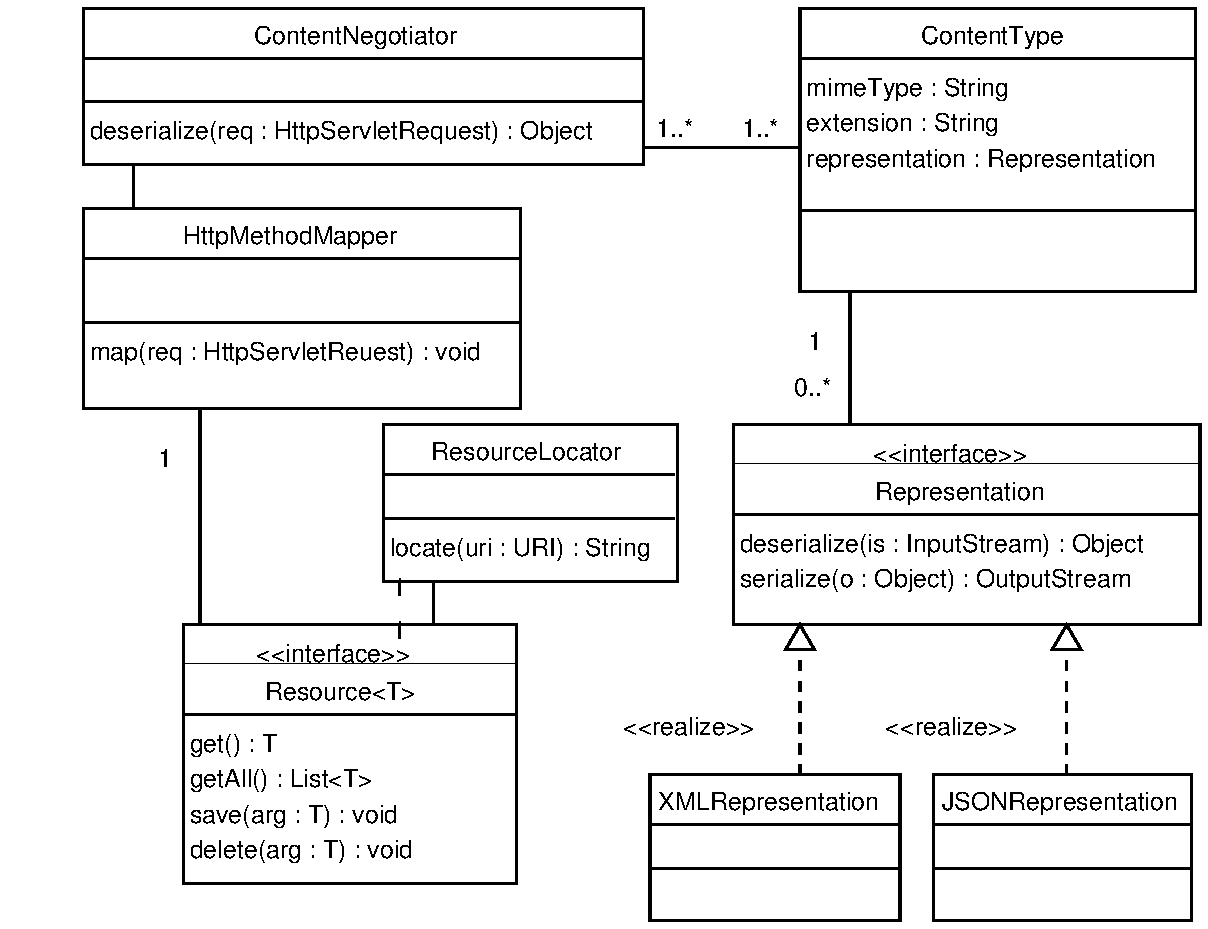
\includegraphics[width=\linewidth]{images/uml/rest}}
	\caption{UML Übersicht des REST Protocol Handler}
	\label{ill:restuml}
\end{figure}

\pagebreak
\subsection{Übersicht}\label{subsec:handlerabstract}
Die folgenden Tabellen \ref{tab:rmiprops}, \ref{tab:xmlrpcprops} und
\ref{tab:restprops} bieten einen Überblick über die wichtigsten Eigenschaften
und Unterschiede der im Verlauf dieses Kapitels vorgestellten \ac{RPC}
Protokolle.

\subsubsection{RMI}

\begin{table}[h]
	\begin{tabularx}{\textwidth}{lX} \toprule
    	\tableheadline{Eigenschaft} &
    	\tableheadline{Beschreibung} 
    	\\
    	\midrule
    	\textsc{Schnittstellenbeschreibung} & Java Interface \\
    	\textsc{Lokalisierung} & \ac{RMI} \ac{URI} \\
    	\textsc{Austauschformat} & Binär (Java Objektserialisierung) \\
    	\textsc{Kommunikation} & Zustandsgebunden \\
    	\textsc{Aufrufform} & Objektorientiert \\
    	\textsc{Fehlerfälle} & Java Exceptions (RemoteException) \\
    	\bottomrule
	\end{tabularx}
	\caption{Eigenschaften von RMI}
	\label{tab:rmiprops}
\end{table}

\subsubsection{XML-RPC}

\begin{table}[h]
	\begin{tabularx}{\textwidth}{lX} \toprule
    	\tableheadline{Eigenschaft} &
    	\tableheadline{Beschreibung} 
    	\\
    	\midrule
    	\textsc{Schnittstellenbeschreibung} & Dokumentation, Introspection \\ 
    	\textsc{Lokalisierung} & Eindeutige \ac{HTTP} \ac{URI} \\
    	\textsc{Austauschformat} & \ac{XML} \\
    	\textsc{Kommunikation} & Zustandslos \\
    	\textsc{Aufrufform} & Prozedural \\
    	\textsc{Fehlerfälle} & Fault Objekte \\
    	\bottomrule
	\end{tabularx}
	\caption{Eigenschaften von XML-RPC}
	\label{tab:xmlrpcprops}
\end{table}

\pagebreak
\subsubsection{REST über HTTP}

\begin{table}[h]
	\begin{tabularx}{\textwidth}{lX} \toprule
    	\tableheadline{Eigenschaft} &
    	\tableheadline{Beschreibung} 
    	\\
    	\midrule
    	\textsc{Schnittstellenbeschreibung} & Methoden aus der \ac{HTTP}
    	Spezifikation \\
    	\textsc{Lokalisierung} & \ac{URI} einer Ressource (z.B. in Hypertext
    	Dokumenten) \\ 
    	\textsc{Austauschformat} & Entsprechend Content Negotiation \\ 
    	\textsc{Kommunikation} & Zustandslos \\
    	\textsc{Aufrufform} & \ac{HTTP} Methoden auf Ressourcen \\
    	\textsc{Fehlerfälle} & \ac{HTTP} Fehlercodes \\
    	\bottomrule
	\end{tabularx}
	\caption{Eigenschaften von REST}
	\label{tab:restprops}
\end{table}